\chapter{Implementation and analysis} 
\label{chap:4}
\noindent In the previous chapter, we mainly identified several subsets of cross-ledger communication schemes and explained the related projects in details. Nevertheless, clear logic levels do not necessarily ensure a good user experience or functional applications. Thus, to evaluate the performance of different protocols or platforms, it is necessary to design and implement appropriate approaches. \\

\noindent Section~\ref{sec:env} introduces the implementation background regarding target blockchain description, test-net setup, and related features. Once we get familiar with the environment, section~\ref{sec:imp} describes the implementation details and working diagram for cross-chain swaps, and some use cases are also mentioned. Then we choose Interledger protocol based application to evaluate the performance for cross-chain transfers, with the working details illustrated in section~\ref{sec:switch}. Section~\ref{sec:sum4} summarizes the results. 

\section{Environment Setup}
\label{sec:env}
\noindent Evaluating all the investigated solutions at this period is unrealistic, for the limited number of blockchains that supported by various platforms, incomplete blockchain plugins designed by protocols, even some of the projects have not implemented for test use so far. Accordingly, at this early stage of cross-chain techniques, the plan is first to implement a basic functional cross-chain swap program, then choose one developed application for source code study. Followed by an analysis of these two solutions from several chosen aspects, such as the complexity of realizing the transaction, safety issues, and future application scenarios.\\
\subsection{Blockchains}
\noindent In these experiments, we aimed at utilizing different cross-chain solutions on two trade parties, which requires the user account setup on those blockchain test-nets. Out of consideration of ensuring the integrity and feasibility of the implementation, we choose Ethereum as the main object blockchain to perform the test.\\

\begin{large}
\noindent \textbf{A. Ethereum}
\end{large}\\

\noindent Ethereum\cite{wood2014ethereum} is an open-source well-known blockchain platform that allows anyone to build and use decentralized applications running through the blockchain technology. Similar to the great significance Bitcoin brought, Ethereum is regarded as the representative of the blockchain 2.0 era. \\

 \noindent The blockchain 1.0 era is usually referred to the development stage of blockchain application represented by bitcoin between 2009 and 2014, where they mainly focus on solving the decentralization of currency and the form of payment. After 2014, blockchain developers are gradually shifting to address the deficiencies of technical and scalability related to bitcoin. In 2014, Vitalik Buterin released Ethereum white paper\cite{buterin2014next}, which introduced smart contracts into blockchain and opened the application of blockchain outside the currency field, thus opening the era of blockchain 2.0.\\
 
 \noindent Ethereum is a programmable blockchain using the Turing-complete scripting language, that enables developers to create a decentralized application that custom complex actions instead of giving users a set of predefined actions. Those applications can be run on Ethereum Virtual Machine(EVM), the core of Ethereum. Advanced and programming friendly is the reason why we choose Ethereum to perform cross-chain solutions.\\
 
\begin{large}
\noindent \textbf{B. Bitshares}
\end{large}\\

\noindent Bitshares\cite{btsintro} is the first delegated proof of stake blockchain created by BM team in 2014. It is an open-source high-performance distributed trading system that supports valuable objects such as cryptocurrencies, legal tender, and precious metals\cite{larimer2013bitshares}. Bitshares blockchain produces the corresponding token BTS for usage in bitAssets system and other finical services featured on the distributed ledger. Compared to Ethereum, Bitshares has much lower transaction confirmation time, and intended to be the commercial exchange platform in the future.\\

\noindent Bitshares also have a convenient idea of mapping account names to addresses, so you can transfer money directly using the name of the account you are applying for, which is a meaningful detail compared to an elaborate list of code addresses. The developed integration library using javascript and HTLC support facilitate my implementation of atomic swaps.\\

\begin{large}
\noindent \textbf{C. Ripple XRP ledger}
\end{large}\\
\noindent Ripple is the world's first open payment network, a peer-to-peer global payment network based on block connectivity. XRP ledger~\cite{xrpledger} presented by Ripple serves as an open-source distributed ledger for real-time financial transactions. As the home of base currency XRP in the Ripple network, it has introduced a unique consensus mechanism RPCA. RPCA~\cite{chase2018analysis} combines the problems of Byzantine generals to get rid of the restriction of consensus through mining and validates and confirm transactions in a short time by voting special nodes.\\

\noindent As another product created by Ripple, XRP ledger is much easier to integrate with Interledger protocol, together will they enable money network interoperability.\\

\begin{table}[H]
\caption{Feature summary of chosen blockchains}
\label{tab:sum}
\begin{tabular}{c|c|c|c}
\toprule
Blockchain                                                             & Ethereum & Bitshares       & Ripple              \\ \midrule
Focus                                                                   & Smart Contract      & DEX & Payment Network\\ \midrule
Consensus Mechanism                                                    & PoW      & DPoS            & RPCA \& FBA         \\ \midrule
Token                                                                  & ETH      & BTS             & XRP                 \\ \midrule
\begin{tabular}[c]{@{}c@{}}Transaction Throughput\\ (tps)\end{tabular} & 15-25    & 3300            & 1500                \\ \bottomrule
\end{tabular}
\end{table}
\noindent Table~\ref{tab:sum} above summarized several important features those three blockchain holds, the data of Ripple and Ethereum throughputs are calculated from the highest  transaction number provided official website transaction charts\footnotemark[1]. And the performance of bitshares is measured by user from test-net\footnotemark[2].

\footnotetext[1]{Ripple:\url{https://xrpcharts.ripple.com/\#/metrics} Ethereum:\url{https://etherscan.io/chart}}
\footnotetext[2]{Bitshares: \url{https://bitsharestalk.org/index.php?topic=23829.0}}

\section{Smart contract}
\noindent Smart contract~\cite{governatori2018legal} is an essential concept and widely used in Ethereum. It is described as a computer protocol to facilitate, verify, or enforce the behavior of contracts digitally. A smart contract allows trusted transactions confirmed without a third-party, and these transactions are untraceable and irreversible. \\

\noindent In Ethereum, smart contracts are written in Solidity language. Solidity~\cite{dannen2017introducing}is one contract-oriented, Turing-complete programming language that mainly consist of four elements: \textit{Contract, Event, Variable, and Function}. \textbf{Event} is one particular part compared to other programming languages. It substituted the Pub/Sub services in Ethereum.\\

\noindent You can set up a smart contract account with functional services by compiling the contract codes and deploying it on the Ethereum network. Once the contract is deployed successfully, the user would get a contract address.  Users could create a transaction containing a payment of ETH to the contract along with other information it may need for the interaction. Similarly, functions and variables could be called afterward. The transaction block would be confirmed to the whole network once the mining computers validate and sign.\\

\noindent By utilizing smart contracts in this implementation, we could simulate cross-chain transactions with Ethereum accounts. Specifically, building the HTLC contract to realize atomic swaps. In the Interledger application, the contract works as the payment channel. Some example codes explanation could be seen in Appendix B ~\nameref{sec:contract}.

\section{HTLC Atomic-swaps implementation}
\label{sec:imp}
\noindent As we discussed in section~\ref{sec:sol}, the most fundamental answer of cross-chain realization is the guarantee of atomicity in transactions. This implementation intended to solve the atomic problem by creating a cross-chain transaction between two parties based on HTLC. The sequence diagram of the cross-chain transaction process is shown in Figure~\ref{fig:success}.\\

\noindent This implementation is performed under the Bitshares private test-net and Ethereum Ropsten test-net environment. BTS holder can only initiate the cross-chain trade in this scenario. This incompleteness is traced back to the HTLC mechanism Bitshares provided, the preimage and hash value are both required when creating the contract. Thus we had to generate unidirectionally.\\

\noindent To ensure the atomicity of the transaction, we recommended and limited the preimage length to be no shorter than 32. In fact, due to the \texttt{Bytes32} format is using in solidity contract creation, specifically, the \texttt{abi.encodePacked(...)} algorithm\footnotemark[1]. This packed algorithm would not treat string shorter than 32 bytes with either zero-padded or sign extended. On the other hand, this limitation brings out stronger hashlock security.\\

\footnotetext[1]{see here: \url{https://solidity.readthedocs.io/en/v0.4.24/abi-spec.html\#abi-packed-mode}}
\noindent Some important functions are explained in~\nameref{app:B} and the whole project can be seen here\footnotemark[2].
\footnotetext[2]{github repo:\url{https://github.com/Fy45/BTS-ETH-atomic_swaps}}

\begin{figure}[H]
    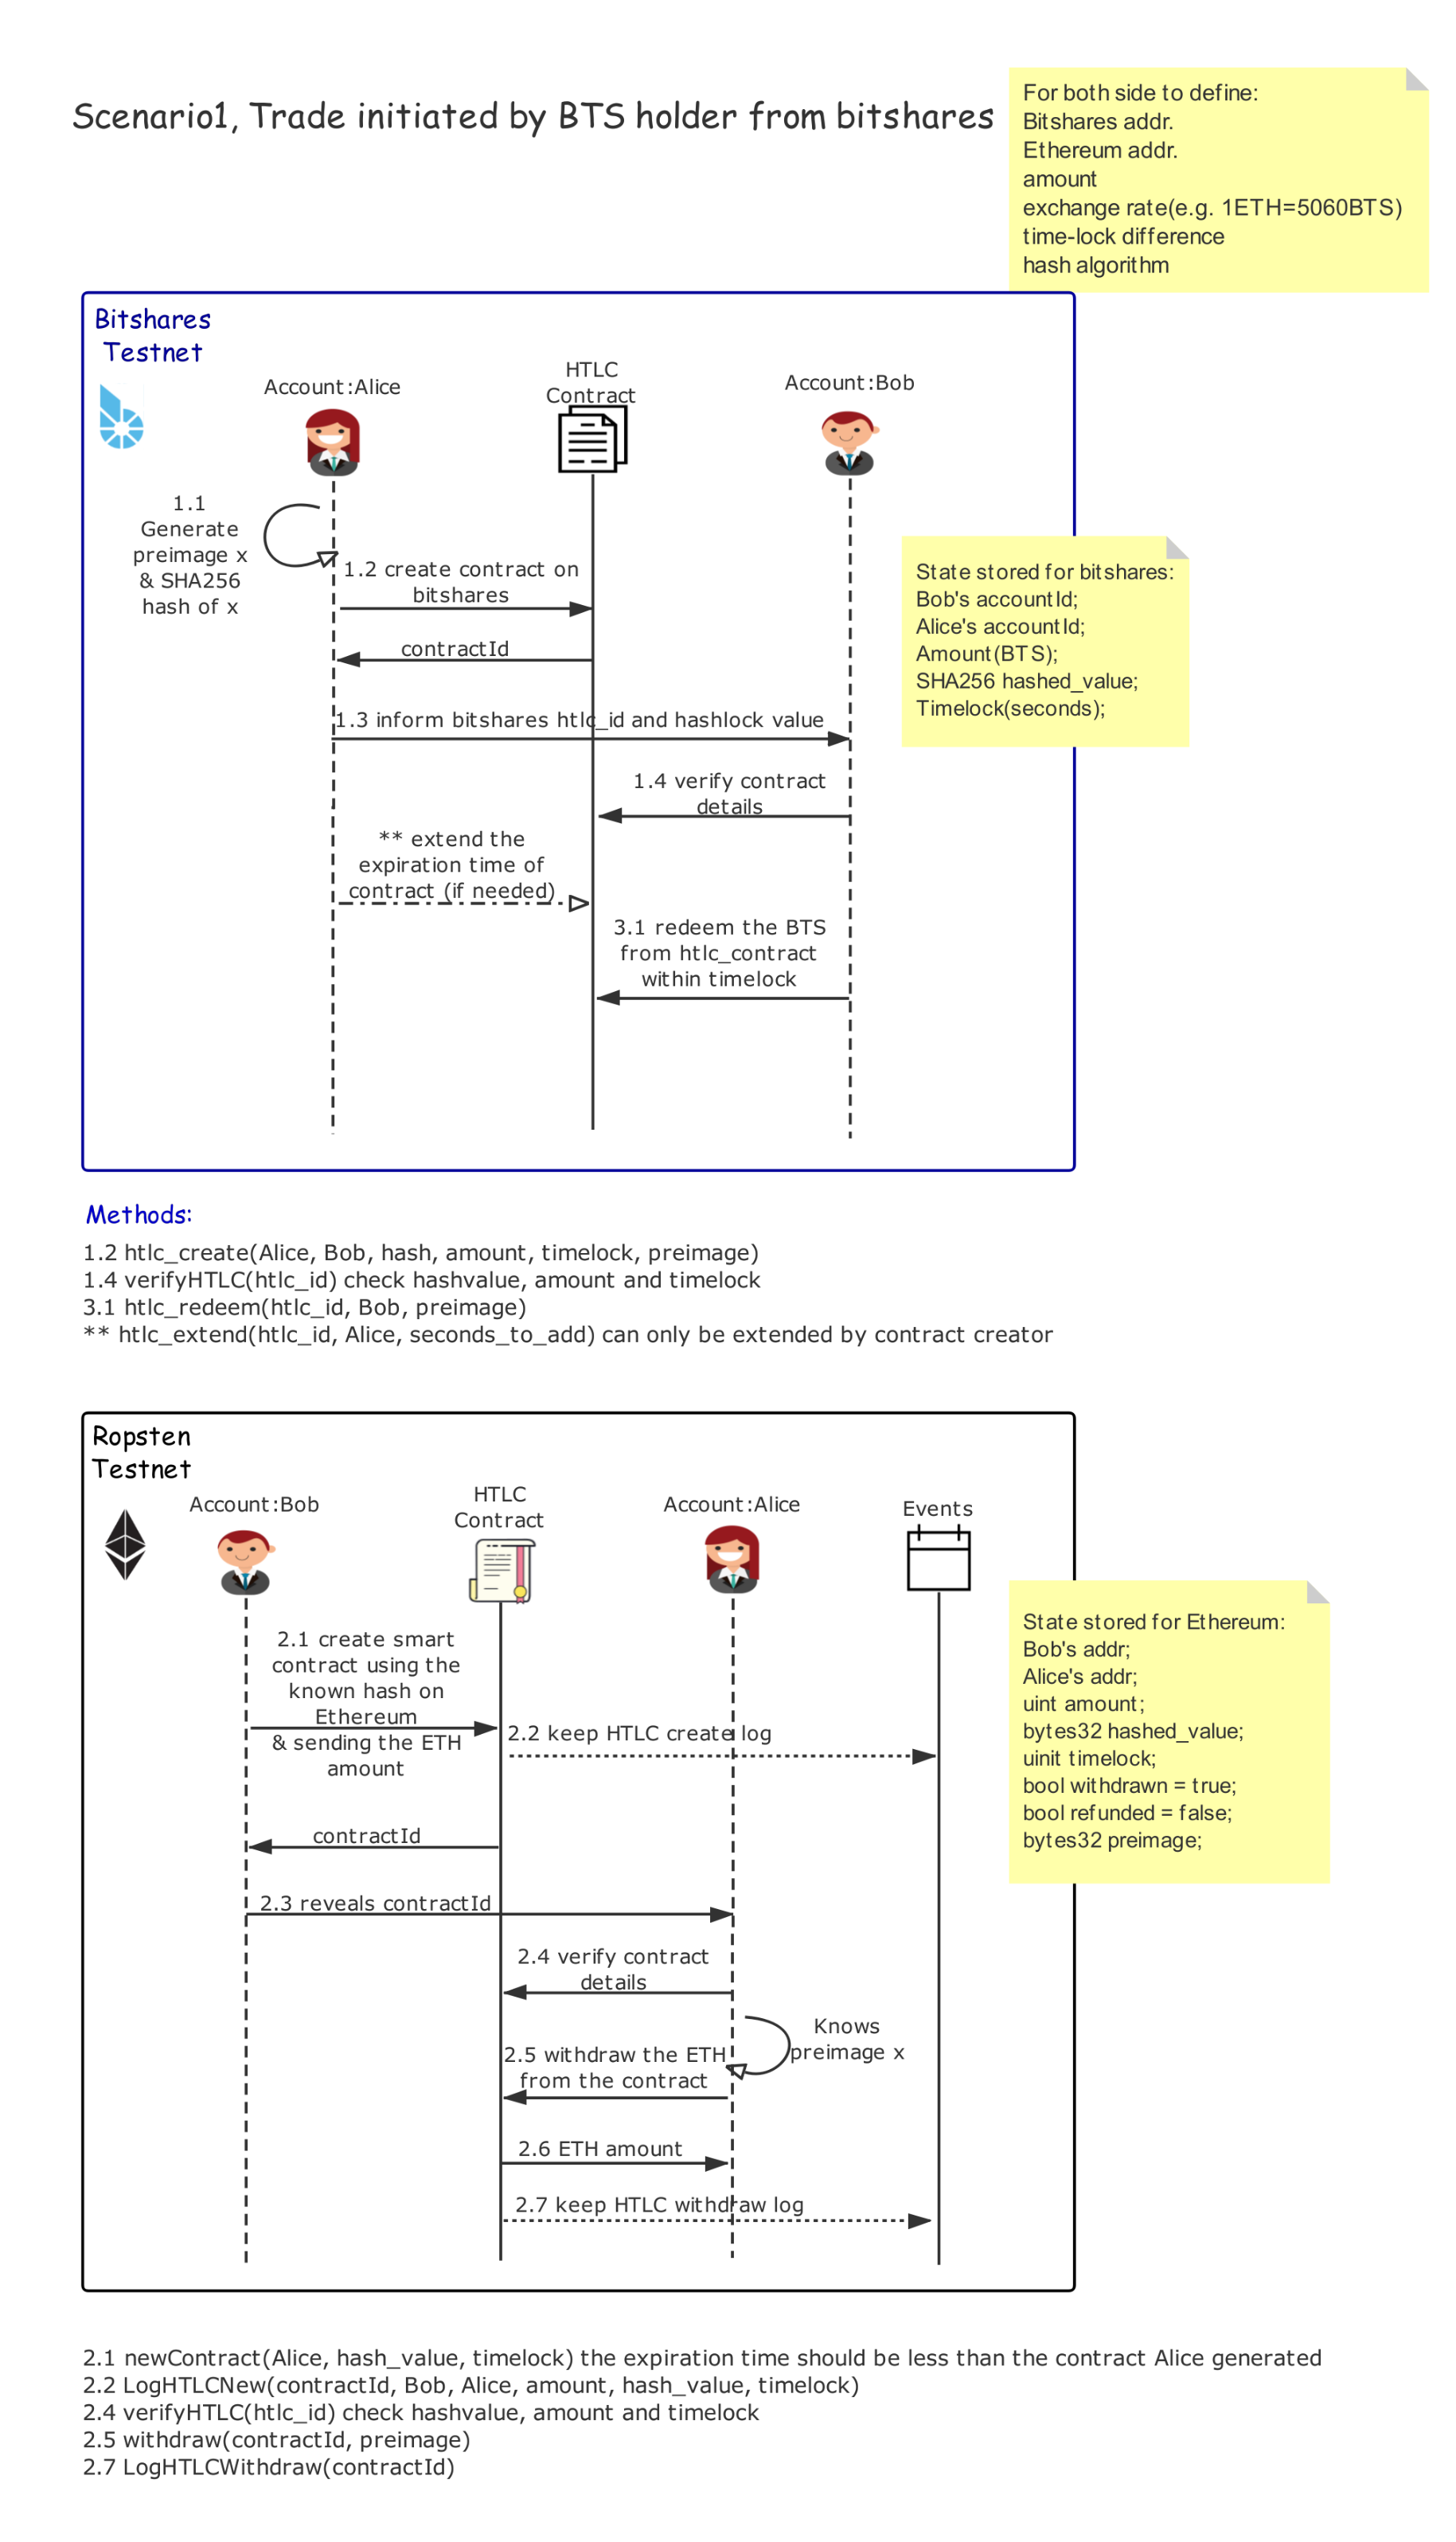
\includegraphics[width=1\textwidth]{./figures/BTS-ETH_diagram}
        \centering
        \caption{BTS->ETH swap diagram}
        \centering
        \label{fig:success}

\end{figure}
\noindent The function of create HTLC, verify the contract details, withdraw the money and refund are realized in this cli application. The following figures~\ref{subfig-1:rebts} and~\ref{subfig-2:reeth} show how a complete cross-chain transaction interacts.\\

\noindent Before the action has been taken. Both parties should agree on the exchange rate and the expiration time offline. As shown in the figure~\ref{fig:success}.
\begin{itemize}
    \item When user Alice chooses to send BTS for ETH, she needs to generate a safety password with fixed length herself first. Along with the counterparty account name, amount and timelock to deploy the contract. The secret should be only known to Alice.  SHA-256~\cite{gallagher1995secure} algorithm is use for calculating Hash value. The transaction is automatically canceled after some period $T$. Then Alice should inform John from Ethereum blockchain with the hashlock value and the BTS HTLC id.
 
    \item John would initiate the contract conditionally on the same hash value he got from Alice, but lock the contract for $T$/2. Thus, it could effectively prevent Alice from doing evil by revealing the secret too late to redeem the BTS. Also, John should notify Alice with the Ethereum contract id.
    
    \item If the contract is executed successfully, both party should verify the timelock, hash value, token amount in the contract by calling \texttt{verifyHTLC(htlc\_id)}. When contract details check out, Alice would reveal the secret to John, which gives her the right to John's ETH and gives John the right to Alice's BTS.

    \item If the contract failed for some reason. Such as information is unmatched with the pre-set value, Alice would not reveal the preimage to redeem the ETH, and John would not give the contract id to Alice. Alternatively, Alice does not reveal the preimage before the time expires, John could call \texttt{refundHTLC(Bob, htlc\_id)} to get ETH back shown in figure~\ref{subfig-3:refund}

\end{itemize}
\noindent Due to different working mechanism in Bitshares and Ethereum, the refund performance differs. Unlike HTLC in Bitshares, which automatically returns the unclaimed amount to the contract creator after time expires, Ethereum handles refund by calling the specific function inside the contract. Moreover, the contract in Bitshares can be extended for a longer time by the sender. 

\begin{figure}[H]
     \subfloat[Complete transaction(ETH->BTS)\label{subfig-1:rebts}]{%
       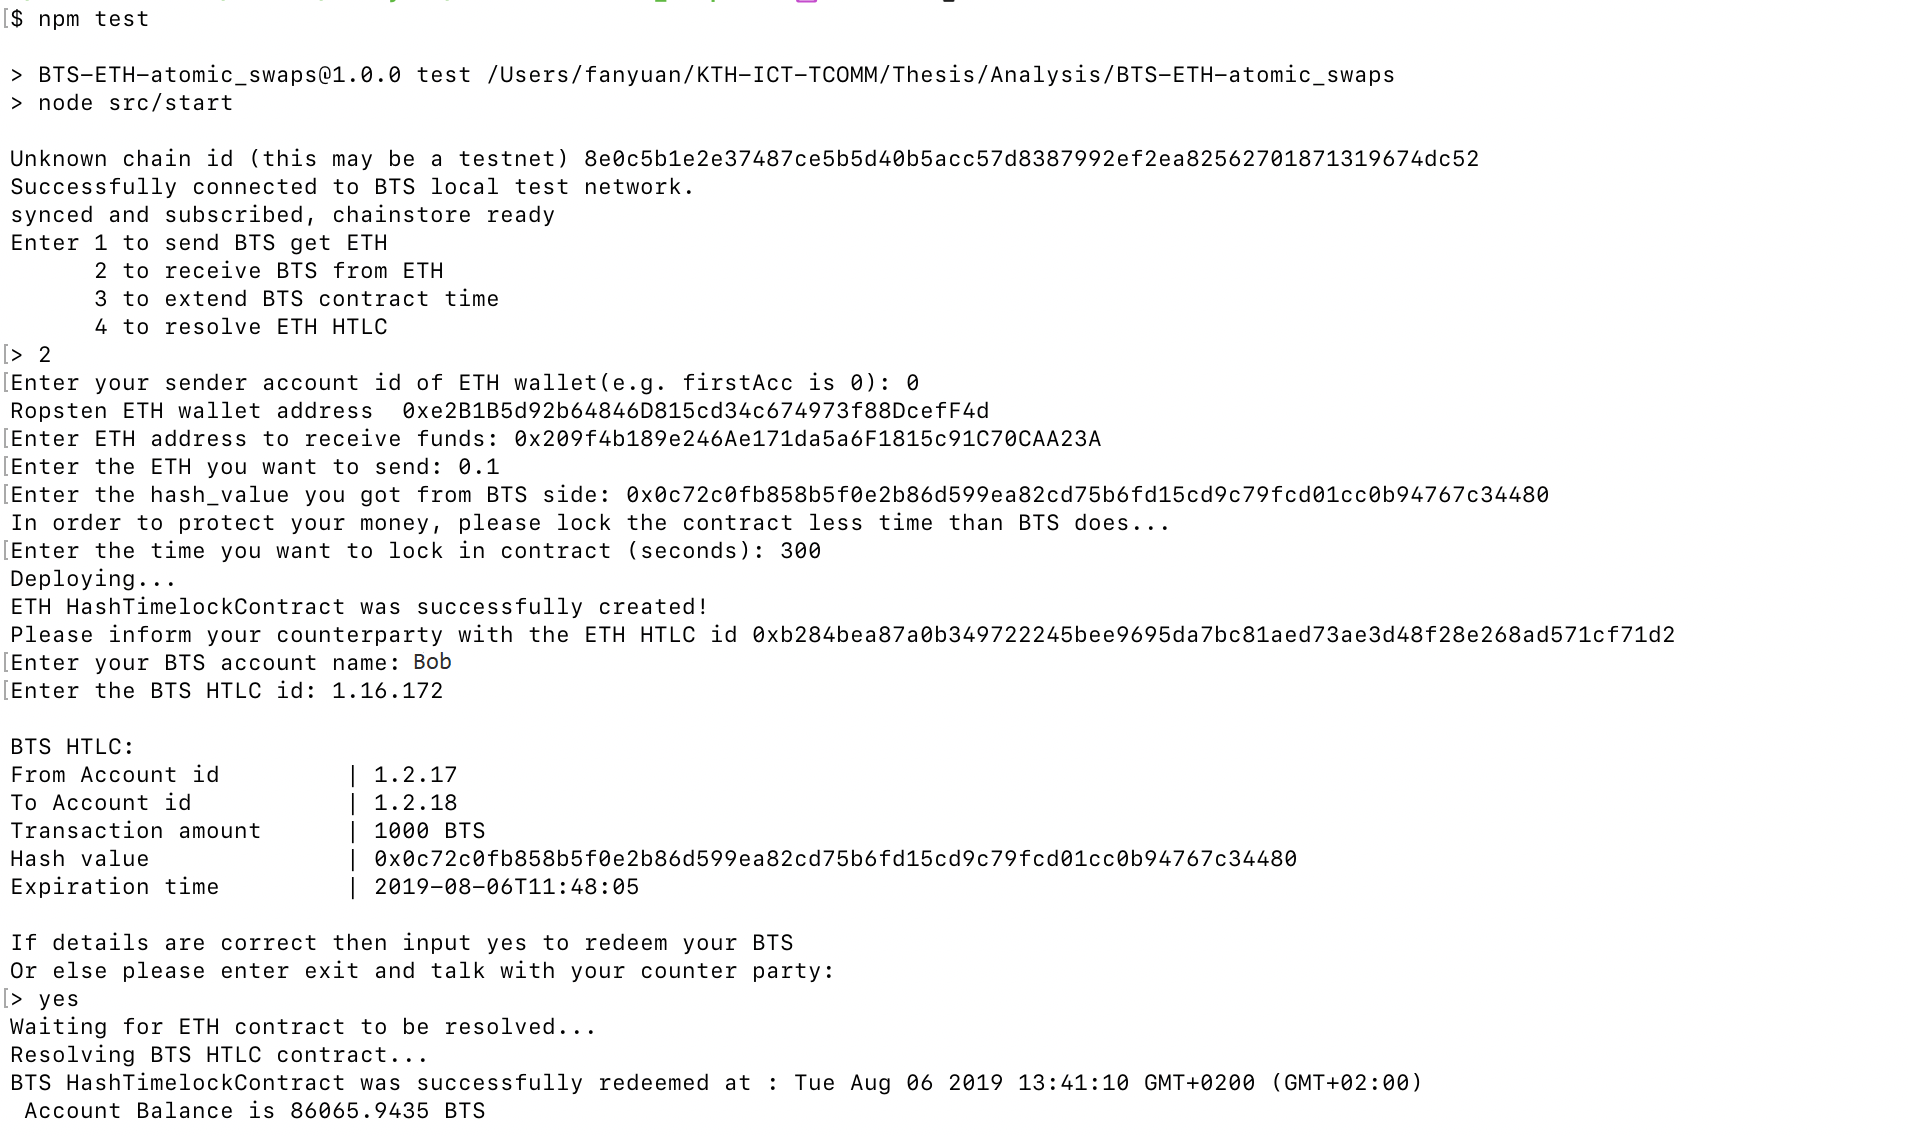
\includegraphics[width=1\textwidth]{figures/screenshots/BTS_redeemed}
     }
     \hfill
     \subfloat[Complete transaction(BTS->ETH)\label{subfig-2:reeth}]{%
       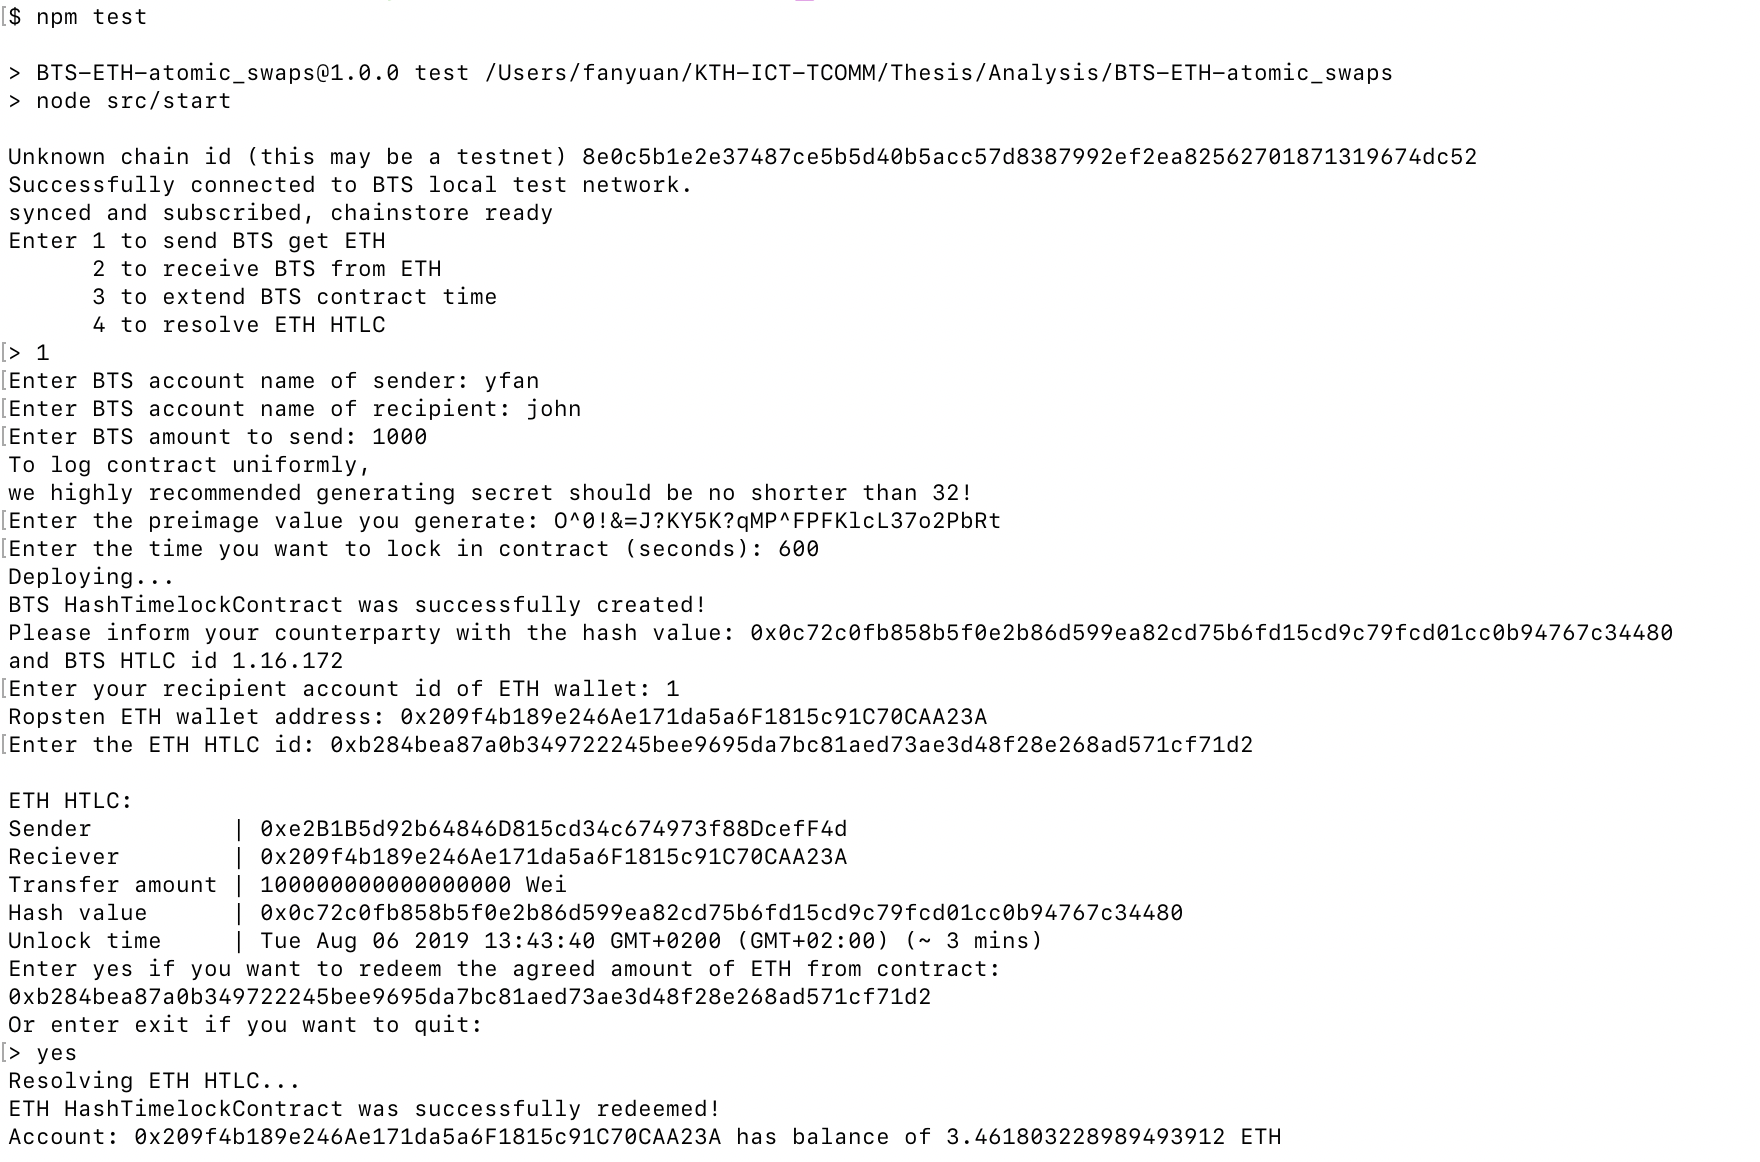
\includegraphics[width=1\textwidth]{figures/screenshots/ETH_redeemed}
     }
     \hfill
     \subfloat[Refund output of ETH\label{subfig-3:refund}]{%
     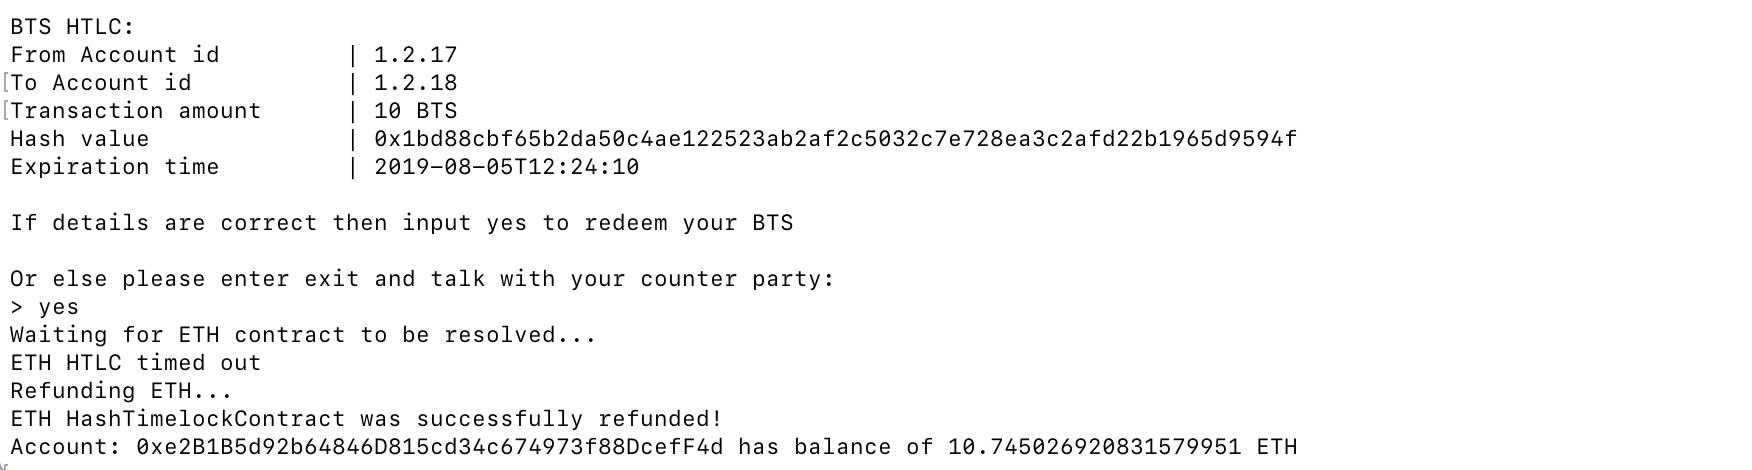
\includegraphics[width=1\textwidth, height=1.2in]{./figures/screenshots/ETH_refund}
     }     
     \hfill
     \centering
     \caption{CLI application outputs}
     \label{fig:out}
   \end{figure}


\section{Interledger switch wallet}
\label{sec:switch}
\noindent Switch is an Interledger wallet shown in Figure~\ref{fig:switch}. It is designed by Kava-labs~\cite{switch} which can be used on the exchange of four types of cryptocurrencies so far. Switch achieved non-custodial cross-ledger transactions by leveraging the stream payment protocol based on ILPv4~\cite{ilpv4}. In this version, ledger-enforced hashlock was removed and change into packetized payment model. The introduction and reasons are illustrated in~\nameref{subsec:stream}.

\begin{figure}[H]
    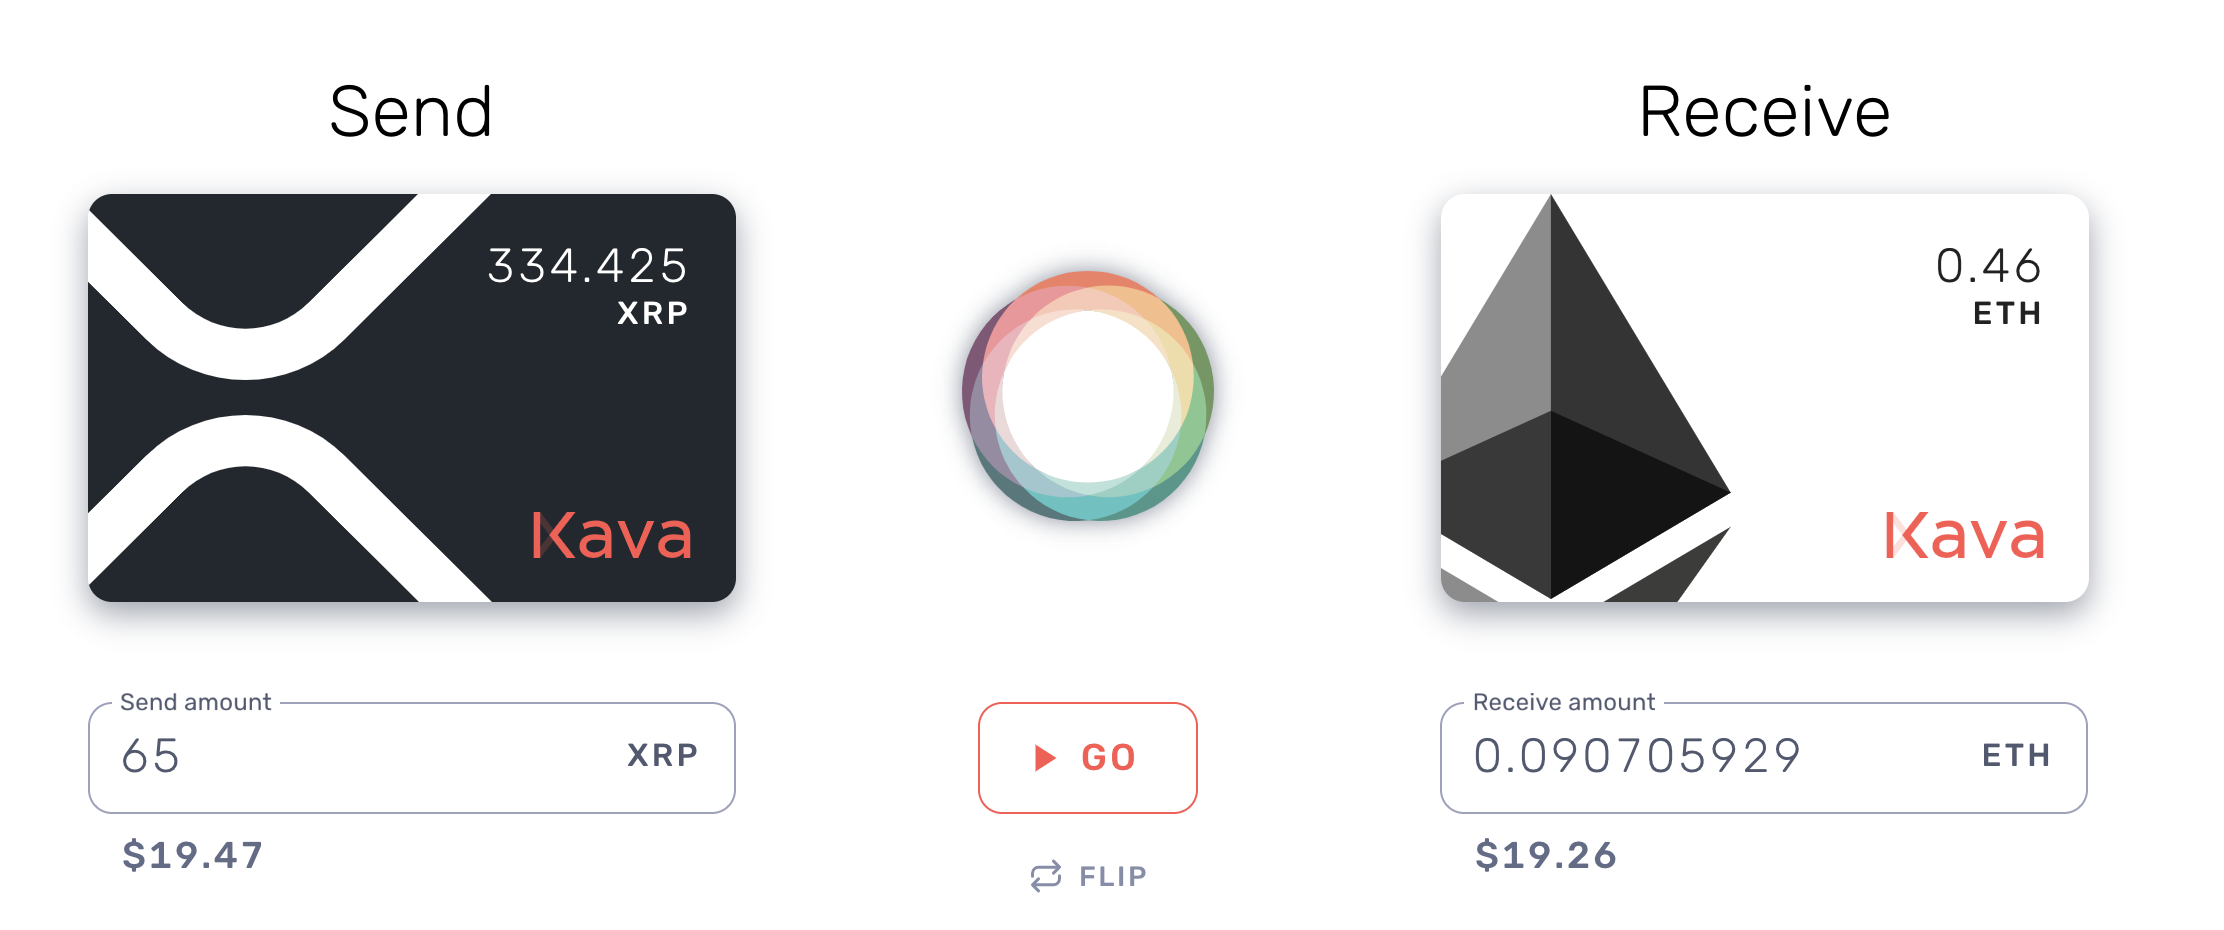
\includegraphics[width=1\textwidth]{./figures/interface}
        \centering
        \caption{Switch wallet interface}
        \centering
        \label{fig:switch}

\end{figure}
\subsection{STREAM payment}
\label{subsec:stream}
\noindent \textbf{STREAM} is an Interledger transport protocol, short for Streaming Transport for the Real-time Exchange of Assets and Messages, is presented by Interledger developer team in 2018~\cite{stream}. This protocol ensures the money and data are sending over ILP packets in a reliable way, often regarded as the TCP in the ILP. \\

\noindent Similar to the Internet network handling the different size of files like streaming media, STREAM protocol adopts the idea of sending the data or money in lots of tiny packets during a short of time. It is efficient since the transaction speed in the blockchain network is dependent on the payment bandwidth, STREAM would automatically adjust the money/data size in each ILP packets to avoid network congestion. Moreover, during one connection, new streams can be open and closed anytime to ensure multiple messages exchanged.\\

\noindent Endpoint in the application based on STREAM protocol could open stream payments, send a specific amount of money through them. The stream abstraction will provide a mechanism to fragment this payment into multiple tiny packets. These packets are authenticated and encrypted by a shared secret. One could close the stream whenever the transaction is complete.\\

\noindent As we discussed in~\nameref{subsec:interledger}, ILP handling the cross-chain payments through a connector/escrow, and the exchange liquidity is also determined by it. So using atomic swaps may cause the problem of floating option~\cite{cryptoeprint:2019:896}. If the exchange rate changes in their favor, they can execute the trade; if the exchange rate goes against them, they can let the timeout expire at no cost, which somehow introduces the counterparty risk. STREAM, on the other hand, set the minimum acceptable amount in each packet, preventing the money claim when the exchange rate is undesired than expected. Build payment channel is also an enhancement to cross-chain interaction since users do not need to wait or pay for the expensive on-ledger transfer every time they had an exchange. Instead, they could call the latest claim to the ledger and get the share amount of money in the channel when they are finished.

\subsection{Work flow}
\noindent Switch is one wallet application that implements the function of assets swaps by making a payment to yourself through a connector. As indicated in RFC~\cite{paymentchannel}, a user could minimize the counterparty risk by using the payment channel and meager in-flight amounts.\\
\noindent The simple workflow is shown in Figure~\ref{fig:flow}. To initiate the asset exchange, user needs to make the deposit to the Interledger wallet from each decentralized ledger first, and start streaming payment, the maximum of M and N is controlled by STREAM protocol, m and n are calculated by the exchange rate connector provided. At the same time, two payment channels are created on each ledger between the kava-lab connector and user account. It should be noticed that the total deposit amount should limit the total exchange amount.

\begin{figure}[H]
    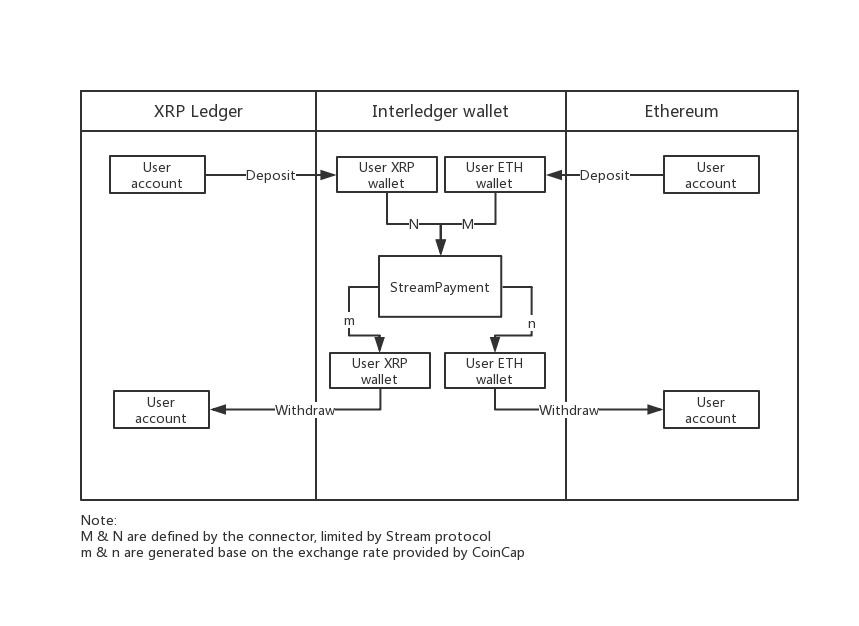
\includegraphics[width=1\textwidth]{./figures/interledgerWallet}
        \centering
        \caption{Exchange Sequence diagram}
        \centering
        \label{fig:flow}

\end{figure}
\noindent Take Ethereum for example, Figure~\ref{fig:dia} illustrates the sequence diagram of how payment channel works.
\begin{enumerate}
    \item After create the payment, the Ethereum account will trigger a micropayment channel through the Machinomy contract\footnotemark[1] with a payment of $X$ ETH for transaction from user account to online-peer, the online-peer defined by connector will also create a channel with $Z$ ETH to user account, the amount $Z$ is a fixed number also defined by connector. The contract will notify both sides with the channel id for interaction.
    \item The user could perform deposit action with $Y$ ETH to channel 1, changing the channel status to ``update'' and channel value to $X+Y$
    \item \begin{enumerate}
    \item If the swap is occurred from ETH to XRP, after one stream payment, the contract will keep the record of the amount of $m$ ETH payment from user account to online-peer in channel 1.
    \item If the swap occurs another way, each stream payment will arouse one deposit of $Z$ ETH to channel 2 to avoid invalid payment due to balance error, and the contract will keep payment record of $n$ ETH from online-peer to user in channel 2.
     \end{enumerate}
     \item To finish the swap, the user will call withdraw from the wallet. Hence the user could claim the correct balance in payment channel 2, update the channel status to ``delete'', and vice versa.
\end{enumerate}
\footnotetext[1]{\url{https://github.com/machinomy/machinomy/blob/97ad47d07a7989b1f38466b1d4b8414e3a978b24/doc/Contract.md}}
\begin{figure}[H]
    \subfloat[ETH->XRP\label{subfig:etx}]{
    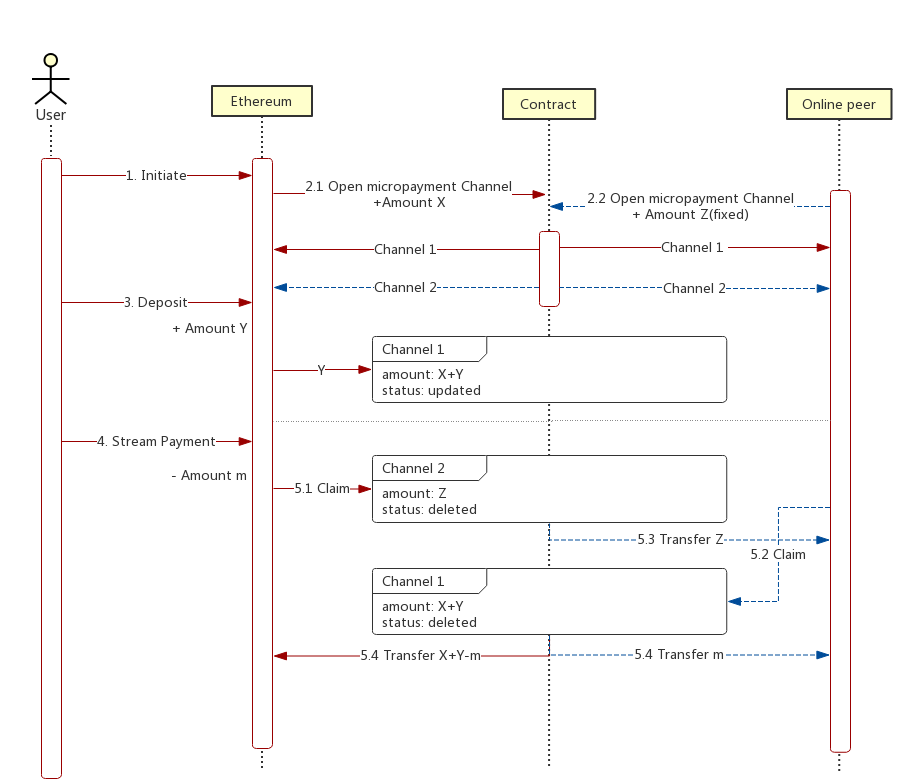
\includegraphics[width=1\textwidth]{./figures/-}}
      \hfill
      \subfloat[XRP->ETH\label{subfig:xte}]{
      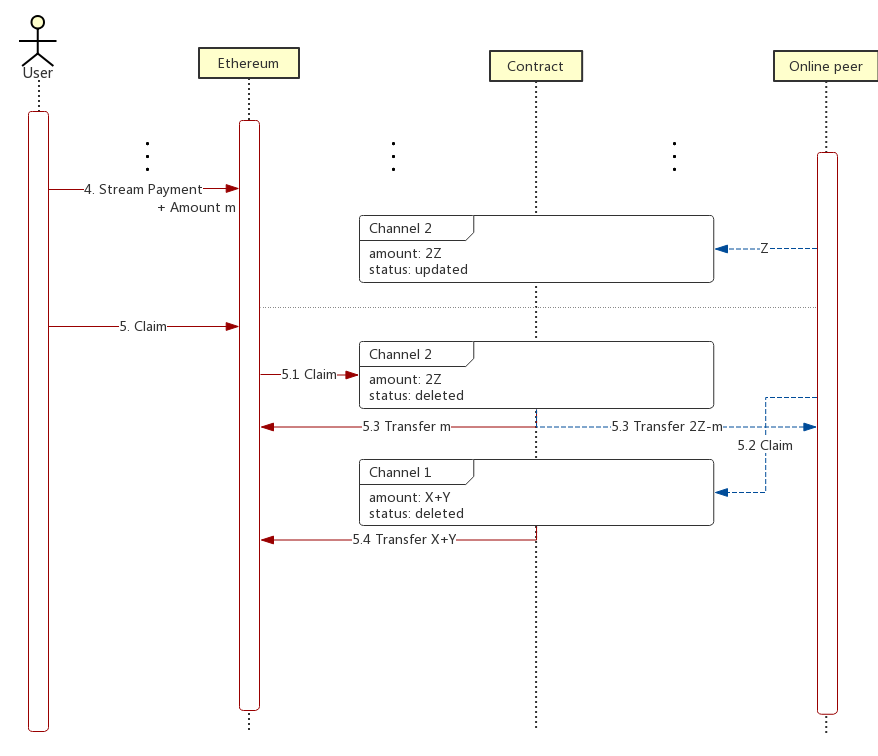
\includegraphics[width=1\textwidth]{./figures/+}}
      \centering
    \caption{Sequence diagram of payment channel}
    \label{fig:dia}
\end{figure}

\section{Summary}
\label{sec:sum4}
\noindent This chapter mainly introduces two implementations of different methods to accomplish the cross-chain transaction. First, we give a brief introduction of the applied ledger features and test environment settings. Then, we implement a simple HTLC atomic swaps framework from Bitshares to Ethereum, present one trade case result. Finally, we studied and tested one developed application integrated with interledger, dig into the working mechanism, and shows the result.
